%! Suppress = NonBreakingSpace

% Add word count of words
%TC:group table 0 1

\chapter{Optimising resource allocation in MEC}
\label{ch:optimising-resource-allocation-in-mec}
In chapter~\ref{ch:introduction}, the problem that this project aims to address was outlined along with a short
description of the proposed solution. This chapter builds upon that, giving a formal mathematical model for the problem
in section~\ref{sec:optimisation-problem}. Section~\ref{sec:auctioning-of-tasks} proposes an auction mechanism in order
to pay servers for their resources in order to deal with self-interested users and as server are normally payed for
use of their services. \\
Using the optimisation problem and auction mechanism from the previous sections, agents for both auction and resource
allocation are proposed, in section~\ref{sec:server-agents}, that learns together to maximise a server's profits
over time.

\section{Resource allocation optimisation problem}
\label{sec:optimisation-problem}
Using the flexible resource principle, the time taken for a operation to occur, e.g.\ loading of data, computing
a program and sending back results, etc, is proportional to the amount of resources allocated to complete the operation.
A modified version of a resource allocation optimisation model can be designed by building upon the formulation
in~\cite{FlexibleResourceAllocation}.

A sketch of the whole system is shown in figure~\ref{fig:system_model}.
The system is assumed to contain a set of $I = \{1,2,\ldots,\left|I\right|\}$ servers that are heterogeneous in all
characteristics. Each server has a fixed resource capacity: storage for the code/data needed to run a task
(e.g., measured in GB), computation capacity in terms of CPU cycles per time interval (e.g., measured in GHz),
and communication bandwidth to receive the data and to send back the results of the task after execution
(e.g., measured in Mbit/s). An example of task could be the analyse of CCTV cameras with 2GB of data, 5GHz of CPU
cycles and 5MB of results. The resources for server $i$ are denoted: $S_i$ for storage capacity, $W_i$ for computation
capacity, and $R_i$ for communication capacity. The system occurs over discrete time steps that are defined as the set
$T = \{1,2,\ldots,\left|T\right|\}$.

\begin{wrapfigure}{l}{0.5\textwidth}
    \centering
    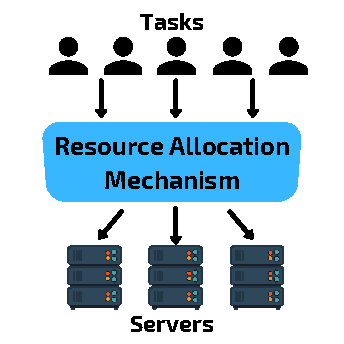
\includegraphics[width=0.5\textwidth]{figures/3_solution_figs/system_model.pdf}
    \caption{System model}
    \label{fig:system_model}
\end{wrapfigure}

The system is also assumed to contain a set of $J = \{1,2,\ldots,\left| J \right|\}$ heterogeneous tasks that require
services from one of the servers in set $I$. To run any of these tasks on a server requires storing the appropriate
code/data on the same server. This could be, for example, a set of images, videos or Convolutional neural network
layers used in identification tasks.\\
The storage size of task $j$ is denoted as $s_j$ with the rate at which the program is transferred to a server at time
$t$ being $s^{'}_{j,t}$. For a task to be computed successfully, it must fetch and execute instructions
on a CPU. We consider the total number of CPU cycles required for the program to be $w_j$, where the number of
CPU cycles assigned to the task at time $t$ is $w^{'}_{j,t}$. Finally, after the task is run and
the results obtained, the latter needs to be sent back to the user. The size of the results for task $j$ is denoted with
$r_j$, and the rate at which they are sent back to the user is $r^{'}_{j,t}$ on a server at time $t$. \\
The allocation of tasks to server is denoted by $x_{i,j}$ for each task, $j \in J$, and server, $i \in I$. This is
constrained by equation~\eqref{eq:server_task_allocation} meaning that a task can only be allocated to a single server
at any point in time.

\begin{align}
    \sum_{i \in I} x_{i,j} \leq 1 && \forall{j \in J} \label{eq:server_task_allocation} \\
    x_{i,j} \in \{0, 1\} && \forall{i \in I, j \in J} \label{eq:server_task_binary}
\end{align}

As the task must complete each stage in series, additional variables are required to track the progress of
each task stage. $\hat{s}_{j,t}$ denotes the loading progress (equation \eqref{eq:loading_progress}), $\hat{w}_{j,t}$
denotes the compute progress (equation~\eqref{eq:compute_progress}) and $\hat{r}_{j,t}$ denotes the sending progress
(equation~\eqref{eq:sending_progress}) of the task. Each of these variables are updated recursively depending
on the progress at the previous time step with the resources allocation. In the compute and sending
progress constraints, the resources allocated are clipped due to requiring the previous stage to finish before the next
stage is started. Progress is limited for each task stage to the total resources required to prevent unneeded
allocation in constraints~\eqref{eq:loading_progress_limit},~\eqref{eq:compute_progress_limit}
and~\eqref{eq:sending_progress_limit}.

\begin{align}
    \hat{s}_{j,t+1} = \hat{s}_{j,t} + s^{'}_{j,t} && \forall{j \in J, t \in T } \label{eq:loading_progress} \\
    \hat{w}_{j,t+1} = \hat{w}_{j,t} + w^{'}_{j,t} \lfloor{\frac{\hat{s}_{j,t}}{s_j}}\rfloor && \forall{j \in J, t \in T } \label{eq:compute_progress} \\
    \hat{r}_{j,t+1} = \hat{r}_{j,t} + r^{'}_{j,t} \lfloor{\frac{\hat{w}_{j,t}}{w_j}}\rfloor && \forall{j \in J, t \in T } \label{eq:sending_progress} \\
    \hat{s}_{j,t} \leq s_j && \forall{j \in J, t \in T} \label{eq:loading_progress_limit} \\
    \hat{w}_{j,t} \leq w_j && \forall{j \in J, t \in T} \label{eq:compute_progress_limit} \\
    \hat{r}_{j,t} \leq r_j && \forall{j \in J, t \in T} \label{eq:sending_progress_limit}
\end{align}

Every task has an auction time, denoted by $a_j$ and a deadline, denoted by $d_j$. This is the time step when the task
is auctioned and the last time for which the task can be completed successfully. Using this deadline constraint can be
constructed such that the sending results progress is finished by at least the deadline time step
(equation~\eqref{eq:deadline}).

\begin{align}
    \hat{r}_{j, d_j} = r_j && \forall{j \in J} \label{eq:deadline}
\end{align}

As servers have limited capacity, the total resource usage for all tasks running on a server must be capped.
The storage constraint (equation~\eqref{eq:server_storage_capacity}) is unique as the sum of the loading progress for
each task allocated to the server. While the computation capacity (equation~\eqref{eq:server_computation_capacity}) is
the sum of compute resources used by all of the tasks on a server $i$ at time $t$ and the bandwidth capacity
(equation~\eqref{eq:server_bandwidth_capacity}) being less than the sum of resources used to load and send results back
by all allocated tasks.

\begin{align}
    \sum_{j \in J} \hat{s}_{j,t} x_{i,j} \leq S_i && \forall{i \in I, t \in T} \label{eq:server_storage_capacity} \\
    \sum_{j \in J} w^{'}_{j,t} x_{i,j} \leq W_i && \forall{i \in I, t \in T} \label{eq:server_computation_capacity} \\
    \sum_{j \in J} (s^{'}_{j,t} + r^{'}_{j,t}) x_{i,j} \leq R_i && \forall{i \in I, t \in T} \label{eq:server_bandwidth_capacity}
\end{align}

\section{Auctioning of Tasks}
\label{sec:auctioning-of-tasks}
While the mathematically description of the problem presented in the previous section doesn't consider any auctions
occurring. In real life servers are normally paid for the use of their resources through auctions as discussed in
Section~\ref{sec:resource-allocation-and-pricing-in-cloud-computing}. However due to the modifications
that this project has to make to the optimisation problems, all of the auction mechanisms discussed are incompatible
due to users not requesting a fixed amount of resources. Nor can the available resources be easily computed as this is
dynamic, depending on the different stages of tasks allocated to a server. Also the modifications effect the algorithms
presented in~\cite{FlexibleResourceAllocation} as they assume that all of the task stages can occur concurrently. This
means that a novel or modified auction mechanism must be used to deal with these changes. Due to the complexities of
devising a new auction mechanism and the large corpus of research on auctions already, an outline of the most common
auctions is presented in table~\ref{tab:auctions_descriptions} with their respective properties in
table~\ref{tab:auction_properties}.

\begin{longtable}{|p{3.5cm}|p{11cm}|} \hline
    \textbf{Auction type} & \textbf{Description} \\ \hline
    English auction & A traditional auction where all participants can bid on a single item with the price slowly
        ascending till only a single participant is left who pays the final bid price. Due to the number of rounds,
        this requires a large amount of communication. \\ \hline

    Dutch auction & The reverse of the English auction, where the starting price is higher than anyone is willing to
        pay with the price slowly dropping till the first participant "jumps in". This can result in sub-optimal pricing
        if the starting price is not high enough or possibly a large number of rounds until anyone bids. Plus due
        the auctions occurring over the internet, latency can have a large effect on the winner. \\ \hline

    Japanese auction & Similar to the English auction, the Japanese auction is instead over a set period of time lets
        bids increasing with the last bid being the winner. Because of this, there is no guarantee that the price will
        converge to the maximum price like the English but the auction has a fixed time length. However factors like
        latency can have a large effect on the winner and resulting price like the Dutch auction. \\ \hline

    Blind auction & Also known as a First-price sealed-bid auction, all participants submit a single secret bid for an
        item with the highest bid winning. As a result, no dominant strategy exist as an agent would wish to bid only a
        small amount more than the next highest price in order to not overpay for an item. But due to there being only
        a single round of biding, latency doesn't affect the winner and can occur over a fixed period of time. \\ \hline

    Vickrey auction~\citep{vickrey} & Also known as a second-price sealed-bid auction, participants each submit
        a single secret bid for an item with the highest bid winning like the blind auction. However the winner only
        pays the price of the second highest bid. Because of this, the dominant strategy (referred to as incentive
        compatibility) for an agent to bid its true value as even if the bid is much higher than all other participants
        its doesn't matter as they pay the minimum required for them to win. \\ \hline
    \caption{Descriptions of feasible auctions for the project: English, Dutch, Japanese, Blind and Vickrey auction}
    \label{tab:auctions_descriptions}
\end{longtable}

\begin{table}[h]
    \centering
    \begin{tabular}{|l|c|c|c|} \hline
        \textbf{Auction}  & \textbf{Incentive compatible} & \textbf{Fixed time length} \\ \hline
        English           & False                         & False            \\ \hline
        Dutch             & False                         & False            \\ \hline
        Japanese          & False                         & True             \\ \hline
        Blind             & False                         & True             \\ \hline
        Vickrey           & True                          & True             \\ \hline
    \end{tabular}
    \caption{Properties of the auctions described in Table~\ref{tab:auctions_descriptions}}
    \label{tab:auction_properties}
\end{table}

The auction properties that this project considers most important in the auction are if it a fixed time length as it is
an Online Auction and Incentive Compatibility such that an optimal strategy actually exists. Because of these two
properties, the Vickrey auction~\citep{vickrey} has been chosen. An additional advantage of incentive compatibility,
is that agents don't need to learn how to outbid another agents, they only needs learn to accurately evaluate each
task allowing agents to learn purely through self-play.

However a modification must be made to the auction due to servers generate the prices for tasks rather than task
suggesting a price to the servers. Because of this, the auction is reversed, such that the bid with the minimum price
wins the task instead of the maximum price. The auction therefore works by allowing all servers to submit their bids for
a task with the winner being the server with the lowest price, but as this is a Vickrey auction, the server actually
gains second lowest price.

\section{Server agents}
\label{sec:server-agents}
Using the optimisation formulation and auction mechanism from the previous two sections, the problem can be modelled as
Markov Decision Process~\citep{Bel} in figure~\ref{fig:mdp_system_model}. This has the advantage of separating out the
auction and resource allocation parts of the problem with separate agents acting for each.
Subsection~\ref{subsec:auction-agents} and~\ref{subsec:resource-allocation-agents} proposes agents
for each of the auction and resource allocation environments respectively.

\begin{figure}[H]
    \centering
    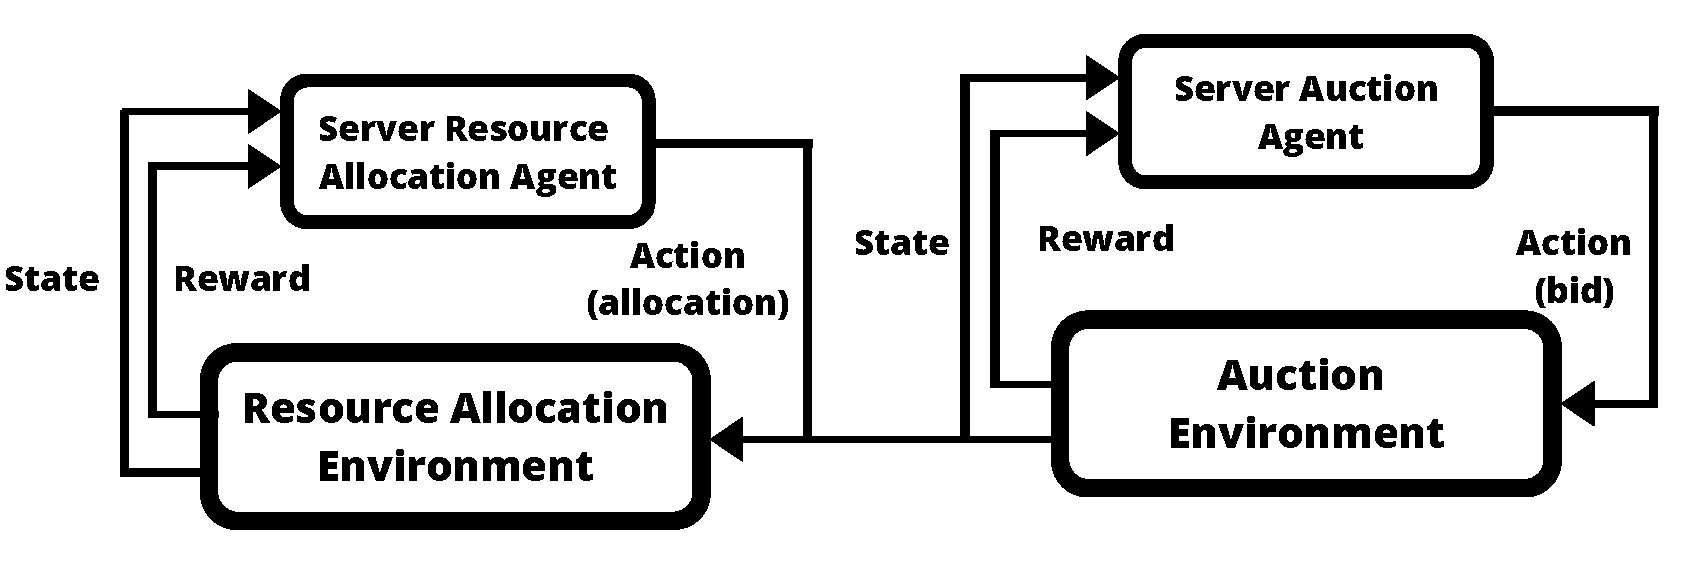
\includegraphics[width=14cm]{figures/3_solution_figs/flexible_resource_allocation_env.pdf}
    \caption{Markov Decision process system model}
    \label{fig:mdp_system_model}
\end{figure}

Due to the exploratory nature of the project, a range of reinforcement learning algorithm and neural network
architectures will be implemented and compared to evaluate the effectiveness of each. These are outlined in
Table~\ref{tab:reinforcement_learning_algorithms} for proposed algorithms and Table~\ref{tab:neural_network_layers} for
networks layers. \\

\begin{longtable}{|p{5cm}|p{10cm}|} \hline
    \textbf{Algorithm} & \textbf{Description} \\ \hline
    Dqn~\citep{mnih2015humanlevel} & A standard deep Q network (Dqn) agent that discretizes the action space with a
        target neural network and experience replay buffer. \\ \hline
    Double Dqn~\citep{doubledqn} & A heuristic for the Dqn that modifies the loss function using the target network
        actions index but the model network value. \\ \hline
    Dueling Dqn~\citep{duelingdqn} & A heuristic for the Dqn that modifies the network to separates the state value
        and action advantages that can help understand the environment. \\ \hline
    Categorical Dqn~\citep{distributional_dqn} & DQN represents the Q value as a scalar value, the Categorical DQN agent
        outputs probability distribution over values which is helpful for environments that are stochastic. \\ \hline
    Deep Deterministic Policy Gradient~\citep{ddpg} & Deep Deterministic Policy Gradient (DDPG) allows for continuous
        actions space, compared to DQN agents that must discretize the action space. This is done through the use of an
        actor and critic network with target networks for each that are updated with a soft target update method. \\ \hline
    Twin delay DDPG~\citep{td3} & Like the Double Dueling DQN agents, Twin deplay DDPG (TD3) includes a couple
        heuristics for the DDPG algorithm. A critic twin is used to prevent the actor network from tricking the critic
        network in evaluating a state's Q value. Another heuristic is the delaying the updates for actor network
        compared to the critic network to allow the critic to out learn the actor to prevent being tricked.\\ \hline
    Td3 Central critic & As there are multiple agents working together, the critic used for all of the agents can be
        same, this is inspired by~\cite{maddpg} which the critic only evaluates the agents private observation not the
        complete information. \\ \hline
    \caption{Table of the Reinforcement Learning algorithms}
    \label{tab:reinforcement_learning_algorithms}
\end{longtable}

\begin{longtable}{|p{3.5cm}|p{12cm}|} \hline
    \textbf{Neural Network} & \textbf{Description} \\ \hline
    Artificial neural networks \citep{ANN} & Originally developed as a theoretically approximation for the brain, it
        was found that for networks with at least one hidden layer, networks could approximate any
        function~\citep{csaji2001approximation}. This made neural networks extremely helpful for cases where it would
        normally be too difficult for a human to specify the exact function, neural networks can be used to find a
        close approximation to the true function through gradient descent. \\ \hline

    Recurrent neural network~\citep{RNN} & A major weakness of artificial neural networks is its use of a fixed
        number of inputs and outputs making it unusable with text, sound or video where previous inputs are important
        for understanding a current input. Therefore recurrent neural network's (RNN) extend artificial neural networks
        to allow for connections to previous neurons to "pass on" information. However this was found to struggle from
        vanishing or exploding gradient during training such that gradients would tended either to zero or infinity
        over long sequences. \\ \hline

    Long/Short Term Memory \citep{LSTM} & Long/Short Term memory (LSTM) aims to remedy RNNs problem of vanishing and
        exploding gradient problems. This is done by using forget gates that determine how much information from the
        last state would get, allowing for more complex information to be remembered over time compared to RNNs. \\ \hline

    Gated Recurrent unit~\citep{GRU} & Gated recurrent unit (GRU) are very similar to LSTMs, except for the use of
        different wiring mechanisms with one less gate, an update gate instead of two forget gates. These changes mean
        that GRUs run faster and are easier to code than LSTMs. However are not as expressive meaning that less complex
        functions can be encoded. \\ \hline

    Bidirectional \citep{Bidirectional} & With RNNs, LSTMs and GRUs, inputs are passed through forward however in
        understanding an input the subsequent inputs are also required. Bidirectional neural network fixed this by
        passes in an input twice, once forwards normally and then a second time in reverse. This allows networks to
        understand the context around an input from both before it and after it. \\ \hline

    Neural Turing Machine~\citep{NTM} & Inspired by computers, Neural Turing Machines build on long/short term memory
        by using an external memory module instead of memory being inbuilt to the network. This allows for external
        observers to understand what is going on much better than other networks due to their black-box nature. \\ \hline

    Differentiable neural computer~\citep{DNC} & An expansion to the Neural Turing Machine that allows the memory
        module to be scalable in size allowing for additional memory to be added if needed. \\ \hline

    Sequence to Sequence networks~\citep{seq2seq} & All networks considered above allow for sequences to be passed in
        while outputting a single output vector. Sequence to sequence network utilise two sub-networks; an encoder and
        decoder. The encoder takes a sequence that is encoded which is outputted to the decoder that then outputs
        another sequence by continually passing in the decoders last input. \\ \hline
    \caption{Neural network layer descriptions}
    \label{tab:neural_network_layers}
\end{longtable}

\subsection{Auction agents}
\label{subsec:auction-agents}
Traditionally pricing mechanisms~\citep{al2013cloud} rely on mixture of metrics: resource availability, resource demand,
quality of service, task resource allocation quantity, etc to determine a price. However
these values are difficult to approximate during the auction for this project. So, due to the complexity of
deriving this function, reinforcement learning will be used to learn an optimal policy for a server to maximise its
profits over time.

\begin{figure}[H]
    \centering
    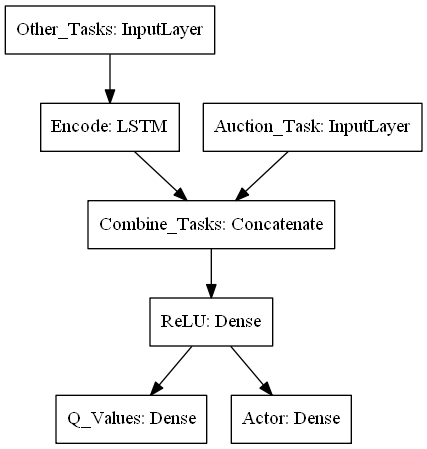
\includegraphics[width=0.5\textwidth]{figures/3_solution_figs/task_pricing_network_architecture.png}
    \caption{Task pricing network architecture}
    \label{fig:task_pricing_network_architecture}
\end{figure}

The network used for the auction must take into account a server's current tasks and the attributes of the task being
auctioned. Because of this, a recurrent network must be used like the RNN, GRU, LSTM and Bidirectional due to the number
of tasks allocated to a server is unknown. For the DDPG, a single ReLU output will be used while a linear Q value output
for DQN agent must be used as shown in Figure~\ref{fig:task_pricing_network_architecture}.

\subsection{Resource allocation agents}
\label{subsec:resource-allocation-agents}
When a new task is allocated to the server or a task completes a stage, server resource need to be redistributed
to the task. While the problem of how to allocation resources isn't as complex as the agent pricing in
section~\ref{subsec:auction-agents}, heuristics are not obvious due knowing how to balance resources usage
between all allocated tasks. Because of this, reinforcement learning agents are proposed to learn this with two
different network structures with a heuristic to simplify the optimal function for agents.

The heuristic is proposed for the network output, such that the network doesn't output the raw
resources allocated for a task but rather a weighted value for the resources needing to allocated for the task.
This has the advantage of being a simpler function to approximate for agents as it is a single positive value but with a
similar expressiveness as an exact resource usage function due to the other values be able to known by the server. This
also avoids the problem of the network either over allocating the resources to tasks or severely under allocating
resources.

\begin{figure}[H]
    \centering
    \begin{minipage}{0.45\linewidth}
        \centering
        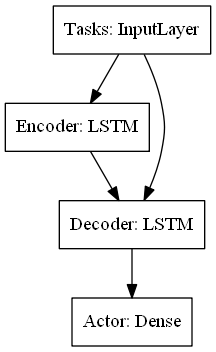
\includegraphics[width=\linewidth]{figures/3_solution_figs/multi_task_actor_weighting_network_architecture.png}
        \caption{Multi-task Seq2Seq actor network architecture}
        \label{fig:seq2seq_actor_network_architecture}
    \end{minipage}\hfill
    \begin{minipage}{0.55\linewidth}
        \centering
        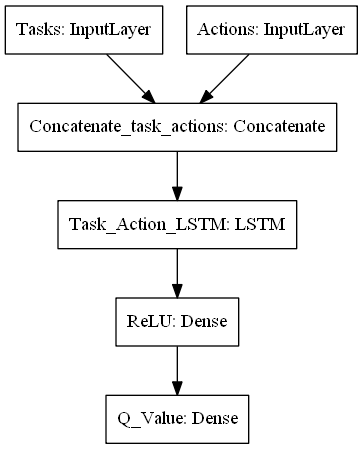
\includegraphics[width=\linewidth]{figures/3_solution_figs/single_task_critic_weighting_network_architecture.png}
        \caption{Multi-task Seq2Seq critic network architecture}
        \label{fig:seq2seq_critic_network_architecture}
    \end{minipage}
\end{figure}

Due to allocating resources to a single task requires being aware of the resource requirements of other tasks, this
effects the network input shape. Two different network structures will be compared, one using a Seq2Seq network such
all tasks are passed in to be encoded with the decode having all of the tasks passed in again generating a sequence of
task weightings. This network architecture is shown in figure~\ref{fig:seq2seq_actor_network_architecture} for the actor
network and figure~\ref{fig:seq2seq_critic_network_architecture} for the critic network. The other network is similar
such that a single task is weighted at a time through passing the single task and the other allocated tasks through the
network as shown in figure~\ref{fig:resource_weighting_network_architecture}. But this requires for each allocated task
for the task to passed through the network however the network can be trained with both deep Q learning and policy
gradient algorithms while the Seq2Seq network must be trained through policy gradient algorithms.

\begin{figure}[h]
    \centering
    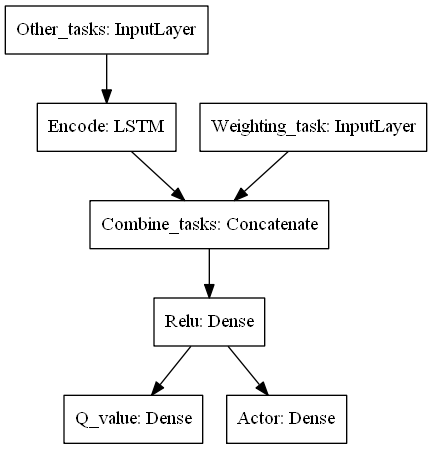
\includegraphics[width=0.5\textwidth]{figures/3_solution_figs/single_task_weighting_network_architecture.png}
    \caption{Single task resource weighting network architecture}
    \label{fig:resource_weighting_network_architecture}
\end{figure}


